\section{Kohn--Sham eigenvalues and the band-gap problem}
\subsection{Physical meaning of Kohn-Sham eigenstates the bandgap problem}

\begin{align} 
    \left(-\frac{\hbar^2}{2m}\nabla^2 + V_{KS}(\vec{r})\right)\psi_i = \varepsilon_i\psi_i
\end{align}

"HF orbitals", "quasi-particles" 

Koopman' theorem in HF: Only the HOMO  $\varepsilon_{HOMO}$ has physical meaning (others $\varepsilon_i$ no)

For $V_{KS}$, it decays to 0 for very large distance. 

\begin{align}
    -\frac{\hbar^2}{2m}\nabla^2 \psi_i = \varepsilon_i \psi_i\\
    \psi_i = c e^{-\sqrt{-\frac{2m\varepsilon_i}{\hbar^2}}r}
\end{align}

At very large distance, only HOMO contributes to the wavefunction density. The density is correct, so HOMO must be correct.

Only in Hatree-Fork:
\begin{align}
    I&= -\varepsilon_{HOMO}\\
    A&= -\varepsilon_{LUMO}\\
    \Delta f &= \varepsilon_{LUMO} - \varepsilon_{HOMO}
\end{align}

People sometimes calculate the band gap by the difference of conduction band minimum (CBM)($\varepsilon_{LUMO}$) and valance band maximum (VBM)($\varepsilon_{HOMO}$), but this is generally not right. It is right when written as I and A.

\subsection{Slater-Janak theorem}
We express the energy functional as:
\begin{align}
    \tilde{E} = \sum_i \left\langle{\psi_i}\left\vert -\frac{-\hbar^2}{2m}\nabla^2 \right\vert{\psi_i}\right\rangle + \int d\vec{r} V_{ext}(\vec{r})\rho(\vec{r}) + E_{Hartree} + E_{XC} \label{eq:KS Functional}\\
    0 \leq f_i \leq 1\\
    \rho = \sum_i f_i \vert \psi_i \vert ^2\\
    \varepsilon_i = \frac{\partial \tilde{E}}{\partial f_i} \label{eq:KS_orbital}
\end{align}

The mathematical expression of KS orbital can be expressed in equation \eqref{eq:KS_orbital}.\\

\textbf{Lemma:} $\displaystyle \frac{\partial F}{\partial x} = \int\frac{\delta F[\rho]}{\partial \rho}\frac{\partial \rho}{\partial x} d\vec{r}$\\
\begin{align}
    \because \lim_{\Delta x\rightarrow 0} \frac{F[\rho+\Delta x \xi(\vec{r})]-F[\rho]}{\Delta x} := \int \frac{\delta F[\rho]}{\delta \rho} \xi(\vec{r}) d \vec{r}\nonumber\\
    \text{Let }\xi(\vec{r})=\frac{\partial \rho(\vec{r},x)}{\partial x}\nonumber\\
    \frac{\partial F}{\partial x}=\int\frac{\partial F[\rho]}{\delta \rho} \frac{\partial \rho}{\partial x} d\vec{r}\label{eq:Functional idt}
\end{align}

Apply \eqref{eq:Functional idt} on \eqref{eq:KS_orbital}, and using \eqref{eq:KS Functional}:
\begin{align}
    \frac{\partial F_{any}[\rho]}{\partial f_i} = \int \frac{\delta F_{any}[\rho]}{\delta \rho} \vert \varphi_i (\vec{r}) \vert ^2 d\vec{r}\\
    \frac{\partial \tilde{E}[\rho]}{\partial f_i}=\left\langle\varphi_i\left\vert-\frac{\hbar^2}{2m}\nabla^2\right\vert\varphi_i\right\rangle+\int d\vec{r}V_{\text{ext}}\vert\varphi_i(\vec{r})\vert^2+\int d\vec{r} V_{\text{Hartree}}(\vec{r})\vert\varphi_i(\vec{r})\vert^2\nonumber\\
    +\int d\vec{r} V_{XC}(\vec{r})\vert\varphi_i(\vec{r})\vert^2\\
    =\left\langle\varphi_i\left\vert -\frac{\hbar^2}{2m}\nabla^2+V_{ext}(\vec{r})+V_{Hartree}(\vec{r})+V_{XC}(\vec{r})\right\vert\varphi_i\right\rangle\\
    =\left\langle\varphi_i\left\vert-\frac{\hbar^2}{2m}\nabla^2+V_{KS}\right\vert\varphi_i\right\rangle=\varepsilon_i\\
    \frac{\partial \tilde{E}[\rho]}{\partial f_i}=\varepsilon_i \label{eq:fraction}
\end{align}
It is obvious that eq \eqref{eq:fraction} is a fraction, therefore, we write:
\begin{align}
    \int \partial \tilde{E}=\int\varepsilon_i \partial f_i\\
    \int_{N-1}^N d\tilde{E}=\int^1_0 \varepsilon_N(N-1+f)df
\end{align}

Define $\varepsilon_i(M)$ as the i-th orbital of the M-electron system.

\begin{align}
    -I = E(N) - E(N-1) = \epsilon_N(N-\delta_I) \times 1
\end{align}
Where $\delta_I \in [0, 1]$ for some $\delta_I$ from Integral Mean Value Theorem

\begin{align}
    \int^{N+1}_N d\tilde{E}&=\int^1_0 \varepsilon_{N+1}(N+f) df\\
    A &= E(N)-E(N+1) = -\varepsilon_{N+1} (N+\delta_A) \quad 0 \le \delta \le 1\\
    \Delta f &= I-A = \varepsilon_{N+1}(N+\delta_A)-\varepsilon_N(N-\delta_I)\\
    &\approx \varepsilon_{N+1}(N) - \varepsilon_{N}(N)
\end{align}
The proof for the continuity of $\epsilon_N$ is left for the readers as an exercise

In general the error is large. For example:
\begin{align}
    \varepsilon_i : \Delta f \approx 1.1 eV\\
    \text{LDA/GGA}: \varepsilon_{CBM} - \varepsilon_{VBM} \approx 0.5/0.6 eV
\end{align}

\textbf{Bandgap discontinuity derivative}
\begin{align}
    \Delta f = I-A = \underbrace{\varepsilon_{N+1}(N+\delta)-\varepsilon_{N+1}(N-\delta)}_{\neq 0}+\underbrace{\varepsilon_{N+1}(N-\delta)-\varepsilon_N(N-\delta)}_{\Delta_{KS}}
\end{align}
It is tricky that the first term is not zero even though $\delta$ is small, the difference of the two energy level is quite large.

\subsection{Physical meanings of KS eigenstates}
As this section is still under developed, the main idea in this paper mainly follows I. P. Perfew: DFT and the bandgap problem, 1986. This section also follow the book "DFT: An approach to the Quantum many body problem" by Dreizier Gross, and the new paper by Perfew et al.: Physics Reveiw A 77 012517 (2008), and Weitao Yang JCP 136, 204111(2012).

Let's consider that our system's overall has a fractional occupied system $N+\omega$ electron:
\begin{align}
    \int \rho(\vec{r}) d\vec{r} = N+\omega \qquad 0\leq\omega \leq 1
\end{align}
Two step minimization gives the mix state:
\begin{align}
    \hat{\rho}=\alpha\vert\phi_N\rangle\langle\phi_N\vert+\beta\vert\varphi_{N+1}\rangle\langle\phi_{N+1}\vert
\end{align}
, with $\alpha+\beta=1$

\begin{align}
    \rho(\vec{r})=\langle r\vert\hat{\rho}\vert r\rangle=\alpha\abs{\phi_N}^2+\beta\abs{\phi_{N+1}}^2\\
    \int \rho(\vec{r}) d\vec{r} = \alpha N+\beta (N+1)=N+\omega\\
    \alpha = 1-\omega\qquad\beta = \omega
\end{align}

Actually, this theory is not rigorous enough. We should set:
\begin{align}
    \hat{\rho}=\sum^{\infty}_{i=1} \gamma_i \bra{\phi_i}\ket{\phi_i}\nonumber\\
    \sum^{\infty}_{i=1}\gamma_i=1\label{eq:tsm1}\\
    \gamma_i\leq 0\label{eq:tsm2}\\
    \int\bra{r}\hat{\rho}\ket{r} d\vec{r} = N+\omega\quad\sum^{\infty}_{i=1}\gamma_i\cdot i=N+\omega\label{eq:tsm3}
\end{align}

Using the two-step minimize approach, we can obtain $E(N+\omega)$ by minimizing \eqref{eq:tsm1}, \eqref{eq:tsm2}, \eqref{eq:tsm3}:
\begin{align}
    E(N+\omega)= \min_{\substack{\eqref{eq:tsm1} \eqref{eq:tsm2}\\\eqref{eq:tsm3}}}\sum^{\infty}_{i=1}\gamma_i E^{GS}(i)
\end{align}

But it turns out that the minimum energy is given by combination of the two states $N$ and $N+1$.


We can do ensemble DFT: Firstly, we minimize all the possible density:
\begin{align}
    E(N+\omega)= \min_{\rho(\vec{r})} \left\{\min_{\substack{\hat{\rho} \rightarrow \rho(\vec{r} )\\\bra{r}\hat{\rho} \ket{r} = \rho(\vec{r})}} Tr[\hat{\rho}(\hat{R}+\hat{V}_{ee}]\int\rho(\vec{r})V_{ext}(\vec{r})d\vec{r}\right\}\\
    =\min_{\rho(\vec{r})}\{\min_{\hat{\rho}\rightarrow\rho(\vec{r})}\{(1-\omega)\langle\phi_N\vert\hat{H}\vert\phi_N\rangle+\omega\langle\phi_{N+1}\vert\hat{H}\vert\phi_{N+1}\rangle\}\}\\
    E(N+\omega)=(1-\omega)E(N)+\omega E(N+1)
\end{align}

Where in the first min $\int \rho(\vec{r}) d\vec{r} = N+\omega$ and in the second one $ \bra{r}\hat{\rho} \ket{r} = \rho(\vec{r}) $

\begin{align}
    \frac{\partial E}{\partial M} = \int \frac{\delta E[\rho]}{\delta \rho} \frac{\partial \rho}{\partial M} d\vec{r}\\
    \because \frac{\delta}{\delta \rho} \left(E[\rho] - \lambda \int \left(\rho(\vec{r}) d\vec{r} - M \right)\right) = 0\\
    \frac{\delta E[\rho]}{\delta \rho}=\lambda\\
    \frac{\partial E}{\partial M}=\lambda\int\frac{\partial \rho}{\partial M} d\vec{r}=\lambda
\end{align}

\begin{figure}[h]
    \centering
    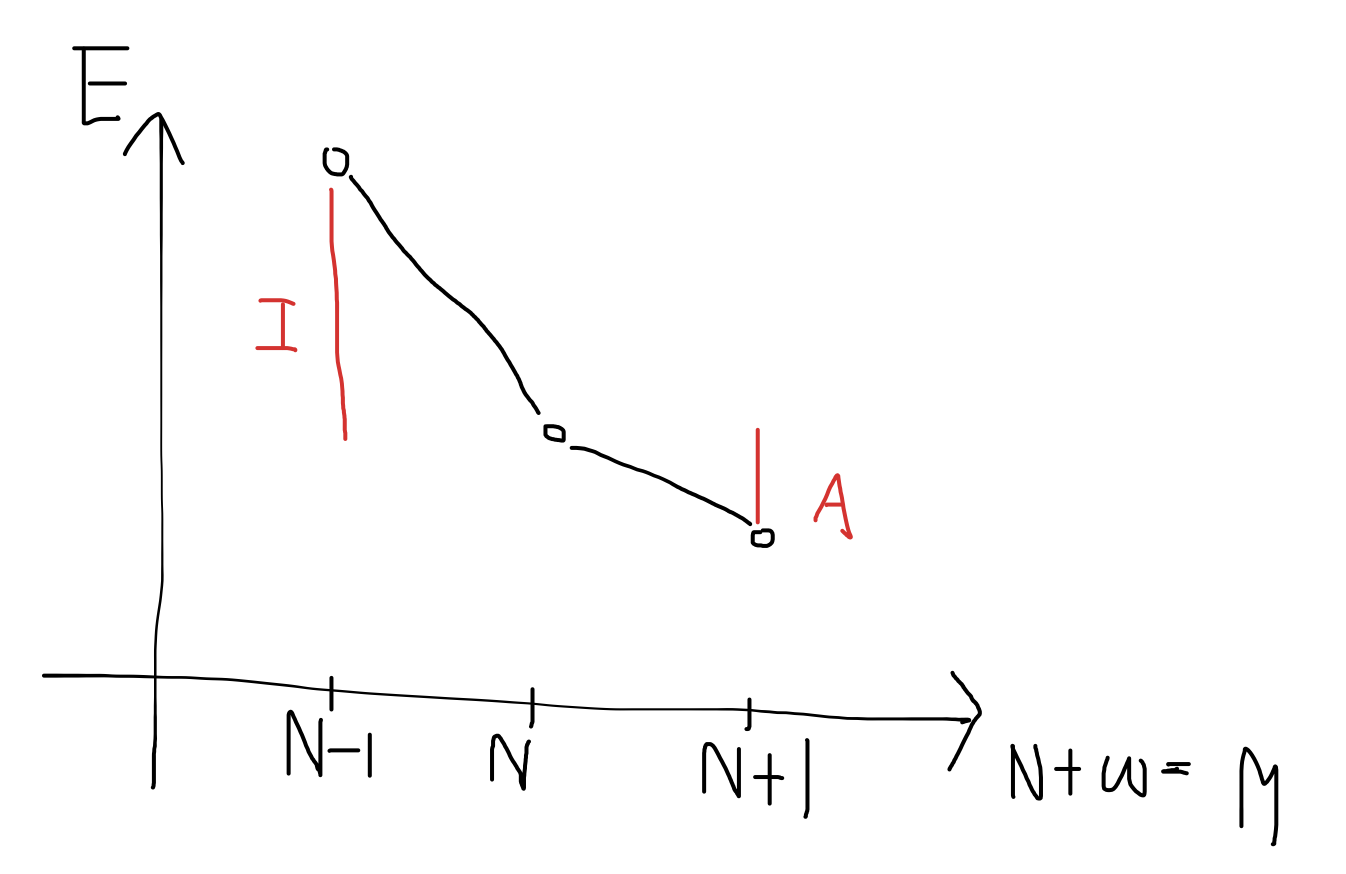
\includegraphics[width=0.5\linewidth]{graph_2.png}
    \caption{Energy vs fractional number of electron}
    \label{fig:fig_2}
\end{figure}

\subsection{DFT and the bandgap problem}
\begin{align}
    \frac{\partial E}{\partial M}=\frac{\partial E[\rho]}{\delta\rho}=\lambda=\mu\\
    \mu=\begin{dcases}
    -I=\varepsilon_N(N-\delta),N-1<M<N\\
    -A=\varepsilon_{N+1}(N+\delta), N<M<N+1
    \end{dcases}
\end{align}

\begin{figure}[t]
    \centering
    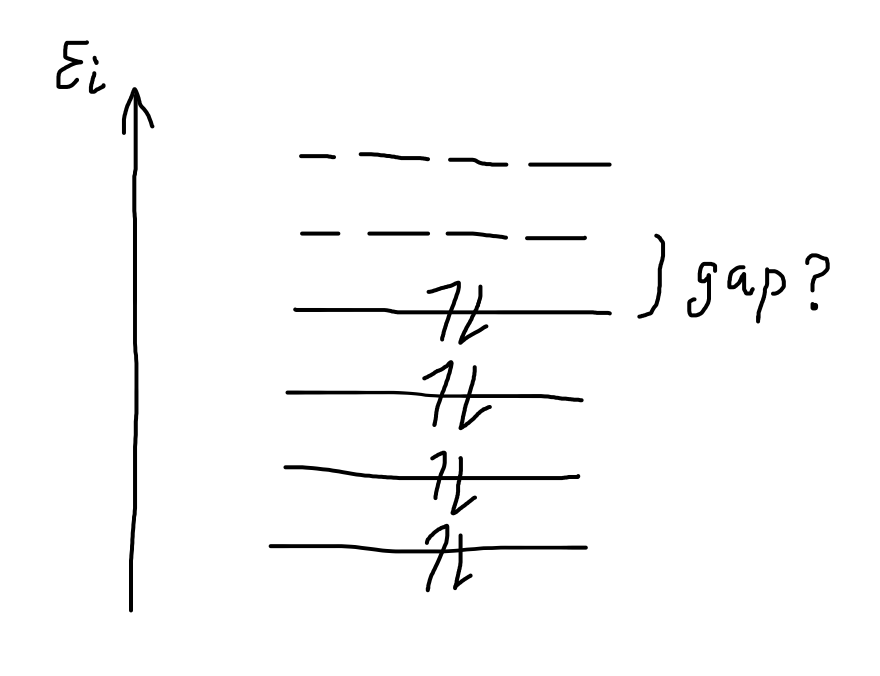
\includegraphics[width=0.5\linewidth]{graph_3.png}
    \caption{}
    \label{fig:figure_3}
\end{figure}

For the real N-electron system:
\begin{align}
    \Delta f &= I-A\\
    &= \frac{\delta E[\rho]}{\delta \rho}\bigg\vert_{N+\delta} - \frac{\delta E[\rho]}{\delta \rho} \bigg\vert_{N-\delta} \qquad \delta\rightarrow0^+\\
    &= \frac{\delta T_{s}[\rho]}{\delta \rho}\bigg\vert_{N+\delta} - \frac{\delta T_{s}[\rho]}{\delta \rho} + \cancelto{0}{V_{ext}\vert_{N+\delta} - V_{ext} \vert_{N-\delta}}\nonumber\\
    &+ \cancelto{0}{e^2\int\frac{\rho(r')}{\abs{\vec{r}-\vec{r'}}}d\vec{r'}\bigg\vert_{N+\delta} - e^2\int\frac{\rho(r')}{\abs{\vec{r}-\vec{r'}}}d\vec{r'}\bigg\vert_{N-\delta}}\nonumber\\
    \nonumber\\
    &+ V_{XC}\vert_{N+\delta}-V_{XC}\vert_{N-\delta}
\end{align}

But the external potential and Hartree energy are continuous, so the discontinuity comes from kinetic energy and exchange correlation energy.


\begin{align}
    \Delta f &= I-A \\
    &= \underbrace{\varepsilon_{N+1}(N+\delta)-\varepsilon_N(N+\delta)}_{\Delta_{KS}} + \underbrace{\varepsilon_{N}(N+\delta)-\varepsilon_{N}(N-\delta)}_{\neq 0}
\end{align}

%The KS-equation can be written as:
%\begin{align}
%    \left(-\frac{\hbar^2}{2m}\nabla^2 + V_{\text{ext}}^{\sigma}(\vec{r})+V_{\text{Hartree}}(\vec{r})+V^{\sigma}_{XC}(\vec{r}) \right)\varphi_i = \varepsilon_i \varphi_i
%\end{align}

Substitute $N=\delta$ and $N-\delta$ on both side and substract the two equation, we can get $\Delta_{XC}=\varepsilon_{N}(N+\delta)-\varepsilon_{N}(N-\delta)$. Therefore, the second term is discontinuity in exchange correlation.

We also have:
\begin{align}
    \Delta_{XC}=V_{XC}\vert_{N+\delta} - V_{XC}\vert_{N-\delta}
    \Delta_{KS}=\frac{\delta T_{s}[\rho]}{\delta \rho}\bigg\vert_{N+\delta} - \frac{\delta T_{s}[\rho]}{\delta \rho}\bigg\vert_{N-\delta}
\end{align}

Noted that $E_{XC}$ cannot be an explicit and differentiable functional of $\rho$.

%\begin{figure}
%    \centering
%    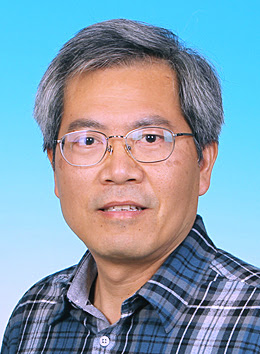
\includegraphics[width=0.3\linewidth]{unnamed.jpg}
%    \caption{A picture of KS}
%    \label{fig:KS}
%\end{figure}

% \begin{figure}
%     \centering
%     
\includegraphics[width=0.5\linewidth]{unknown.png}
%     \caption{Scarlett jeh jeh}
%     \label{fig:siu_sei}
% \end{figure}

\newpage
